\documentclass[../thesis.tex]{subfiles}
\begin{document}
\chapter{Algorithms Experimental Results}
\label{ch:experimentsalgos}

\section{Results - Efficacy of More Popular Algorithms}

The test suite runs all of the algorithms discussed above on a subset of stocks and generates profit figures for different denominations of stocks purchased. For every buy signal generated, the strategies ran on purchasing 10, 100, and 1000 stocks at a time. The strategies were implemented in Python and accessed stock data stored in csv files. The implementation leveraged Pandas Dataframes to store and manipulate the stock data. Pandas is a python data analysis package and is perhaps the most powerful open source data analysis or manipulation tool available. See Section 7.1 for pseudocode of each strategy's implementation.  The best way to understand how effective a particular strategy is to compare against a baseline, which is discussed above, helping us analyze the effectiveness of each strategy.   

\subsection{Momentum Strategies}

Standalone momentum strategies as a whole very rarely beat out the baseline measure. Figure 9 displays the results of AAPL, GOOG, HAS, QCOM, and AMD when using SMA, EMA, Bollinger Bands, and RSI. Only a few stocks had any strategies beat the baseline. One was GOOG, with both Bollinger Bands and RSI outperforming the baseline profit significantly. AMD for both SMA and EMA proved to be effective as well. However, for most it was more profitable to simply just buy and hold over the period. Figure~\ref{MOMENTUMfigure} demonstrates this poor performance. The baseline bar chart on the right side of the graph outperforms nearly every strategy. This however seems counterintuitive, as we should be generating profitable buying and selling trading signals with all of the computation, but that is clearly not the case.  Clearly, these strategies aren't viable as standalone trading algorithms. Now we will discuss why we observed overall poor performance.

The dual moving average algorithm when applied to both SMA and EMA isn't particularly effective. Due to the nature of SMA, which generally looks at long periods of time to highlight trends, this can induce a lagged effect to the buy and sell orders. A lagged effect in the context of moving averages is that the current moving average doesn't react to the current trend because of this longer observation window, often making this method ineffective. This lagged effect can be fixed by looking at an Exponential Moving Average analysis \cite{Ehlers}. However, unlike the literature suggests, in practice this doesn't translate to profit. AAPL nearly doubled its profit from using the exponential window that removes the lagged effect yet still had 2.53\% less returns than the baseline. While as a whole the strategy was more effective than SMA and did come closer to baseline performance, it rarely ended up beating it. This suggests that these indicators should be looked at in a different, combined context where multiple indicators could provide more robust trading signals. See the following section for discussion. 

With Bollinger Bands, buy and sell signals are still reliant on changes in rolling average prices. However, because of the incorporation of standard deviation, this strategy uses volatility in the market to further base buy and sell decisions. While a significant portion of the chosen stocks didn't end up actually out performing the baseline, a majority of them were within 1-2 percent performance of the baseline. 33\% of stocks tested on the strategy out performed each of its own baseline measure of buying and holding a specific denomination of shares throughout the entire period. Most notably, GOOG outperformed the baseline by 2.77\% while the implementations of SMA and EMA had abysmal performances of -30.25\% and -19.41\% respectively. While still not a passable standalone algorithm, the improvement over SMA and EMA is encouraging.

RSI takes advantage of over-purchasing or overselling of securities to predict convergence back to the mean. So, this strategy does take advantage of mean reversion. Unfortunately, most RSI implementations didn't outperform the baseline. The performance was comparable to EMA but slightly worse, as we see less stocks beating out the baseline. GOOG beat the baseline by 12.88\% while on the other hand DIS massively underperformed and posted a -7.08\% performance. 

\begin{figure}[h]
\centering
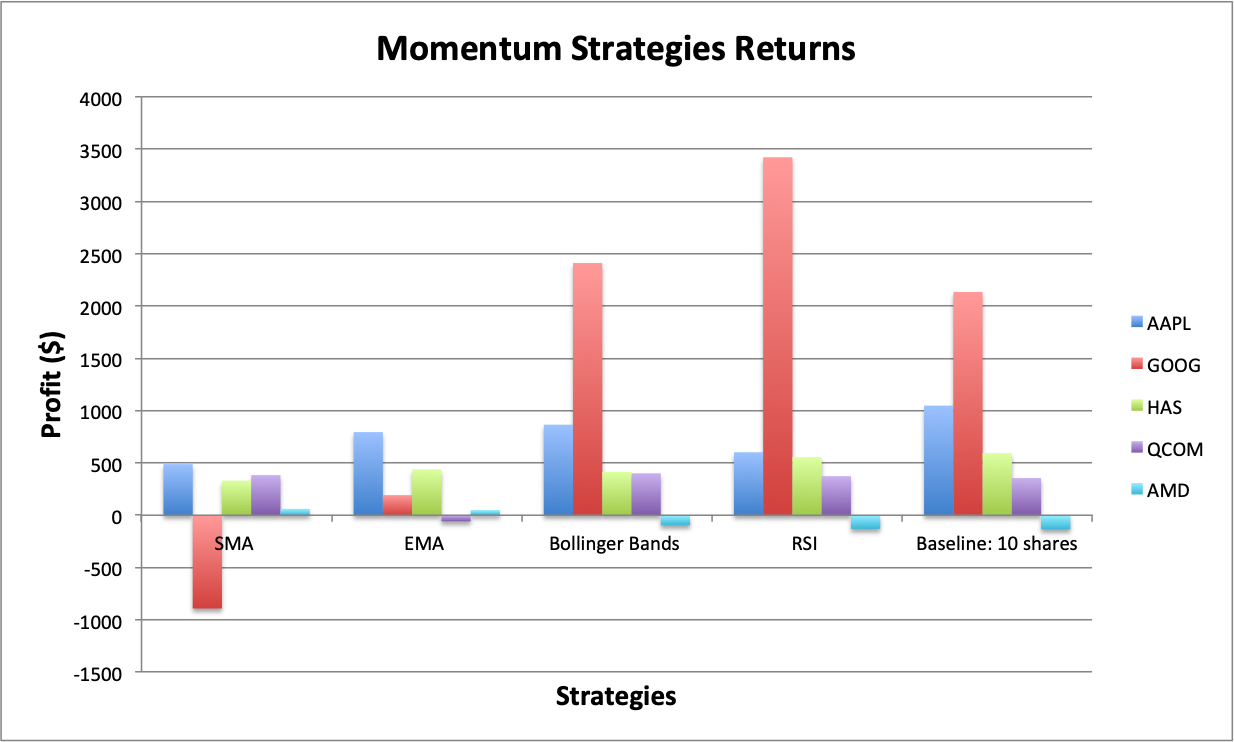
\includegraphics[width=.9\textwidth]{momentumstrategiesreturns.png}
\caption{Momentum Strategies Results  \label{overflow}}
\label{MOMENTUMfigure}
\end{figure}

\subsection{Combination Momentum Strategies}

The RSI and MACD combined implementation performed incredibly well. The most notable performances were from AAPL and HD. When purchasing 1000 shares at each buy signal, AAPL out-gained the baseline by \$9070  while HD had \$4990 of profit with the strategy while the baseline lost \$3750. Of all 30 stocks tested, only 3 stocks ended up with negative profit at the end of the day. AXP is a good example - generating a loss of \$1300 more than the baseline. With enough capital, this strategy could be used to generate incredible returns on a daily basis. Figure~\ref{RSIMACDRESULTSfigure} shows this strong performance. The green bar - the profit of the strategy buying or selling 1000 shares at a time, beats out the correspond baseline purple bar for every single stock, giving truly significant results. 

This algorithm generates incredibly robust buy signals and frequent sell signals which can nearly guarantee gains after buy signals. Therefore, utilizing strategies where 1000 shares of a given stock can generate massive profits with less risk of massive losses. It is also important that each transaction purchases a large amount of shares because it is necessary to offset the transaction cost charged by brokers. However, rather than focusing on individual stocks over time, this combination strategy is best implemented over a pool of multiple stocks because it isn't uncommon for days to generate absolutely no buy signals.

\begin{figure}[h]
\centering
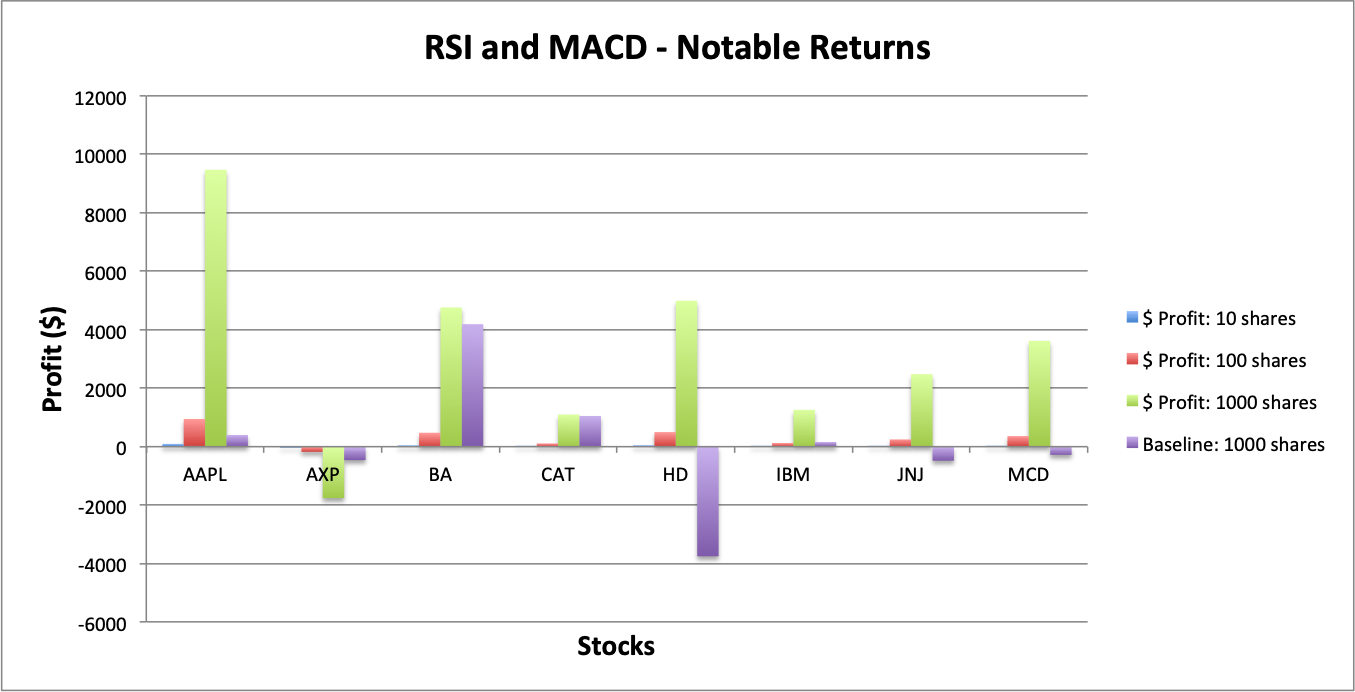
\includegraphics[width=.9\textwidth]{rsimacdresults.png}
\caption{RSI and MACD strategy   \label{overflow}}
\label{RSIMACDRESULTSfigure}
\end{figure} 

\subsection{Pairs Trading}

Just like the above strategy, our pairs trading implementation performed incredibly well. Compared against the baseline of SPY, a mutual fund that is the industry standard for baseline comparison of AT strategies, this strategy has amazing performance. When using AMD against SBUX, the strategy profited 2143.28\%. QCOM and SBUX performed similarly - culminating in 1748.06\% returns. However, even the lowest performing combination, AMD and VOD, beat out the baseline by over 138\%. Figure~\ref{PAIRSRESULTSfigure} shows these truly astounding results. Furthermore, this strategy would need to be tested on a larger pool of stocks, as only 5 combinations of stocks were cointegrated enough to justify trading together. 

This highlights a common trend. More involved strategies that use multiple measures or inputs always perform better than single measures and nearly always beat the baseline. Just like the combination momentum strategies, the results are incredible. With both pairs trading and as well as the above strategy, someone who implements either strategy could make incredible profits. The barrier to entry however for individuals to truly generate these massive profits, is being able to access up to the minute stock data. All data found via the internet or Quandl is delayed by upwards of 20 minutes, which can make the difference between thousands of dollars and profits and thousands of dollars of losses. However, because pairs trading uses closing prices, one wouldn't have to pay for the end of day closing data.

\begin{figure}[h]
\centering
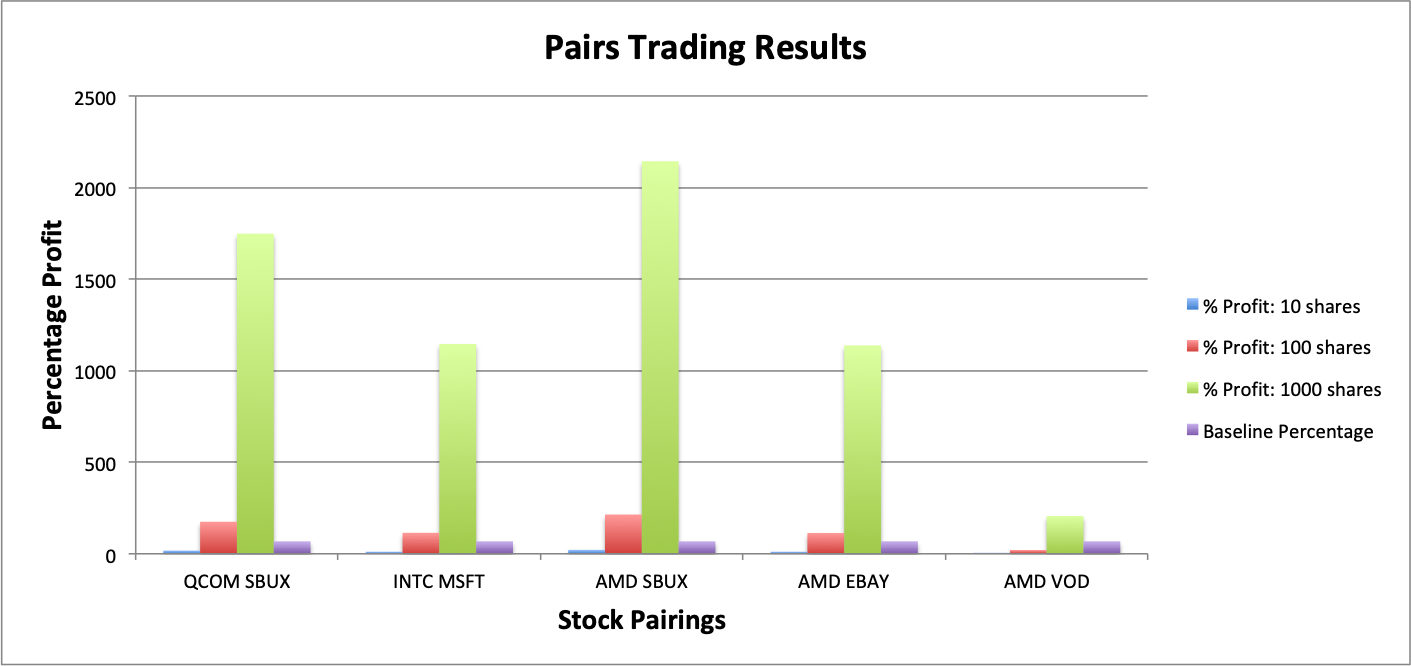
\includegraphics[width=.9\textwidth]{pairstradingresults.png}
\caption{Pairs Trading Results \label{overflow}}
\label{PAIRSRESULTSfigure}
\end{figure}

\section{Twitter Sentiment Strategy}

We find each of our different twitter sentiment strategies to have mixed results. Different models have differing effects on various stocks. As discussed below, we generally see for all of the models that they consistently beat the baseline on stocks with poor performance during the time period. Typically, stocks that have a strong baseline performance are rarely beaten by any of our strategies. However as a whole, each specific model generates some extraordinary individual performances for the strategy above the baseline. We don't find that one machine learning algorithm has consistent notable good performance. The results have somewhat random performances on each model for different stocks. This lack of consistency is due to the difference in data and sentiment for each stock. Because we fit the model for each stock on each machine learning algorithm, it would be highly improbable to see one model give consistent results due to the random nature of market movement. 

As a whole, it would be difficult to trade using this entire group of tested stocks, but our testing reveals some encouraging results. Trading on this twitter sentiment strategy would certainly come with lots of risk and trading is at the individuals discretion. However, individual results that beat the baseline by nearly 100s of percentage points offer some starting points for making a live trading implementation. Specifically, using our deep learning strategy on SBUX nets a 54.5\% profit over the trading period, while the baseline \textit{buy-and-hold} nets a loss of 23.7\%. Or we could look to implement the stacking lenient strategy for MNST, as our strategy nets a 50\% profit while the baseline nets a loss of 31.2\%. Another encouraging result worth pursuing in live trading is the extended model decision tree algorithm for AMD. For this particular stock, our algorithm nets a 629.1\% profit, almost doubling the baseline's already impressive 307.3\% profit. Our research shows that starting with these 3 stocks and the associated strategies would be a great start to a sample portfolio.

\subsection{Basic Model}
Our most basic model has the worst performance of any of the tested strategies. Only a few of the stocks tested had truly notable performances. Figure~\ref{simpleresults} shows the performance of a selection of stocks that were tested. We rarely find any machine learning algorithm actually beat the baseline. Only 29.4\% stocks tested ended up beating the baseline. The vast majority of stocks tested performed like FB, with all 4 of our machine learning algorithms generating profits slightly below or right at the baseline. However, some did actually find success. QCOM's random forest regressor beat the baseline by \$379.5 whereas SBUX's decision tree classifier beat the baseline by \$428.32. These results suggest, even with a handful of stocks showing profitable trading margins, that we need to utilize a model that has more inputs so our model can more effectively predict following day stock price movement. We find improvement across the board by adding more inputs into the model as seen in the next subsection. 

\begin{figure}[h]
\centering
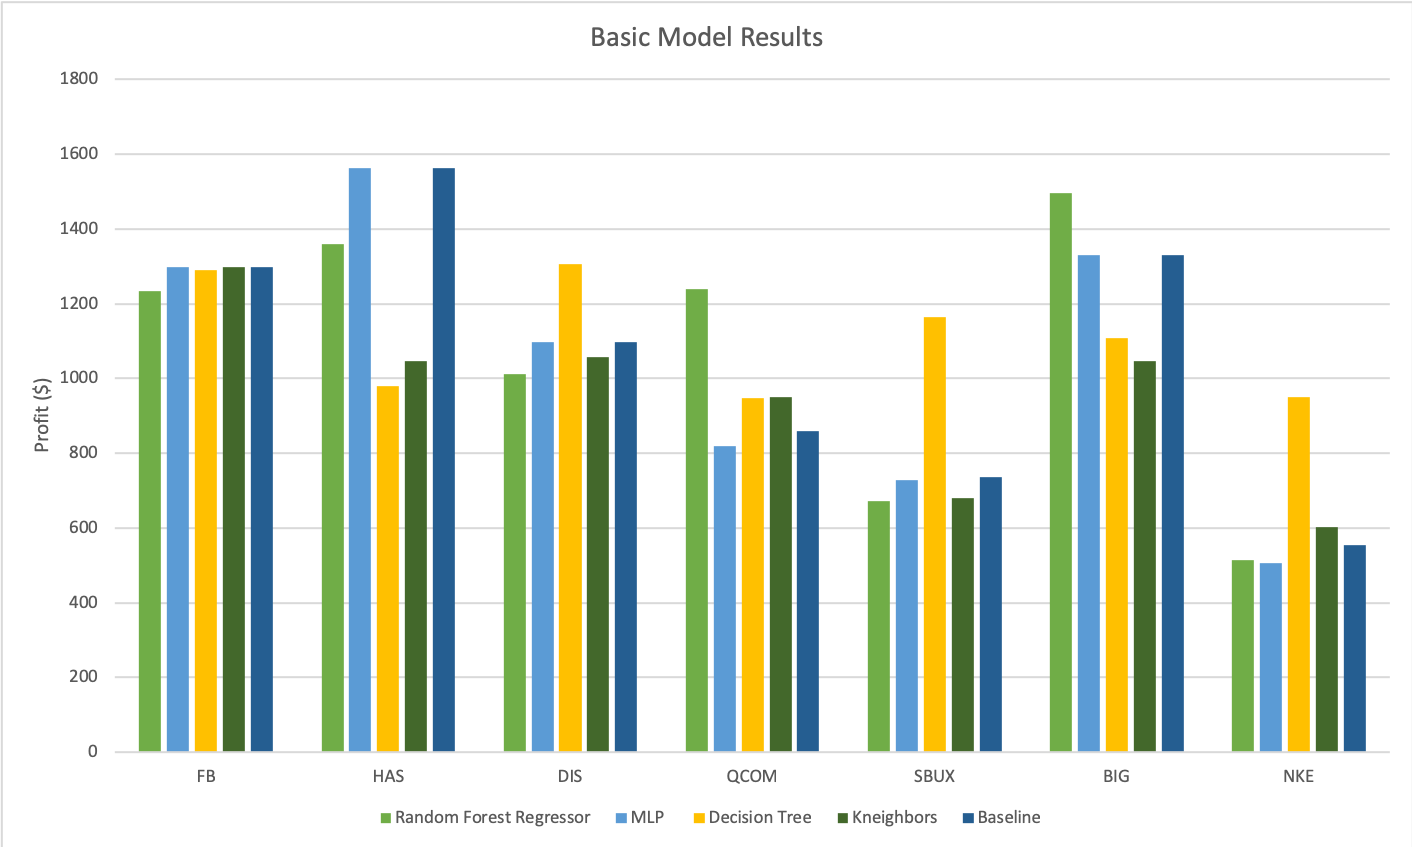
\includegraphics[width=.9\textwidth]{BasicModelResults.png}
\caption{Basic Model Results \label{overflow}}
\label{simpleresults}
\end{figure}

\subsection{Extended Model}
Our extended model that adds additional twitter features for the input has an overall improvement over the basic model that only takes in closing price and twitter sentiment. Figure~\ref{complexresults} shows the performance of a selection of stocks that were tested. We find that 82.4\% of the stocks tested have a particular algorithm that beats the baseline. This is an improvement of 53\% moving to a model with more inputs. This means that including features such as amount of tweets and retweets are useful for stock trading. Specifically, AMD has the most remarkable performance, with the decision tree classifier generating 629.1\% profit and doubling the baseline profit. We find MNST to also have impressive returns with this model. the decision tree classifier generates a 79\% profit while the baseline nets a loss of 31.2\%. The random forest regressor of BIG generates 88.7\% profit, beating the baseline by 55.7\%. These returns for specific models on specific stocks are significant enough to implement for a realtime for-profit trading algorithm, showing that twitter sentiment can be used to aid stock trading.

\begin{figure}[h]
\centering
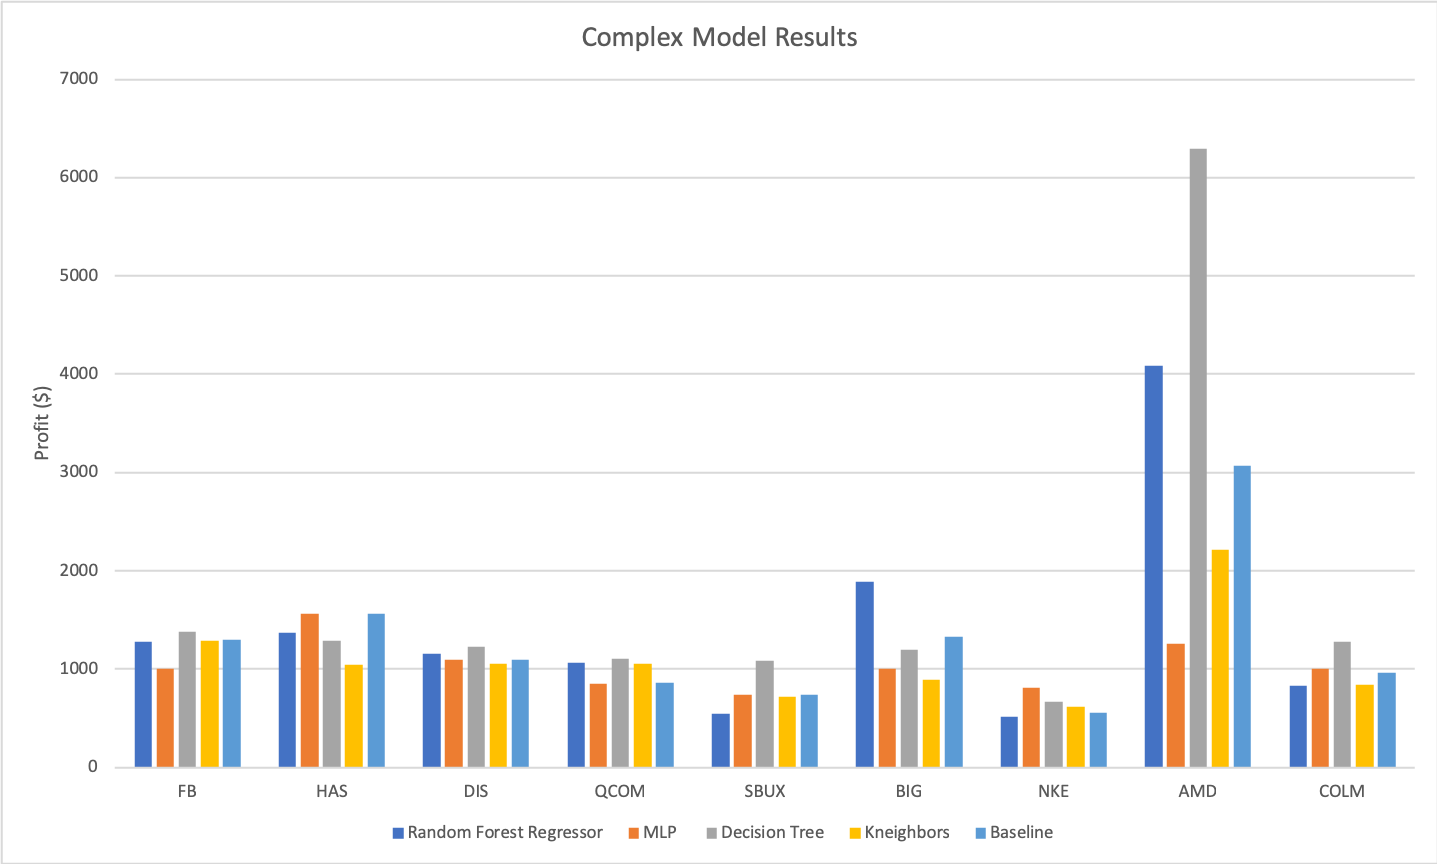
\includegraphics[width=.9\textwidth]{ComplexModelResults.png}
\caption{Extended Model Results \label{overflow}}
\label{complexresults}
\end{figure}

\subsection{Stacking Model}
Our stacking model that aggregates all of our various machine learning models into one buy or sell signal doesn't perform as well as the extended model, but handily beats the basic model. Figure~\ref{complexresults} shows the performance of a selection of stocks that were tested. We find that 58.8\% of the stocks using the conservative strategy beat the baseline, while only 29.4\% of the lenient strategy beat the baseline. In particular, MNST has fantastic performance, netting a 50\% profit while the baseline nets a loss of 23.7\% while using the lenient strategy. EBAY's conservative strategy has a 6.9\% return while the baseline has a 39.5\% loss. In these results, the stocks that end up beating the baseline are generally because of the baseline losing money over the trading period. While a few stocks do end up beating a high performing baseline, this strategy like others using twitter sentiment, performs much better when the stock does poorly over the trading period. 

\begin{figure}[h]
\centering
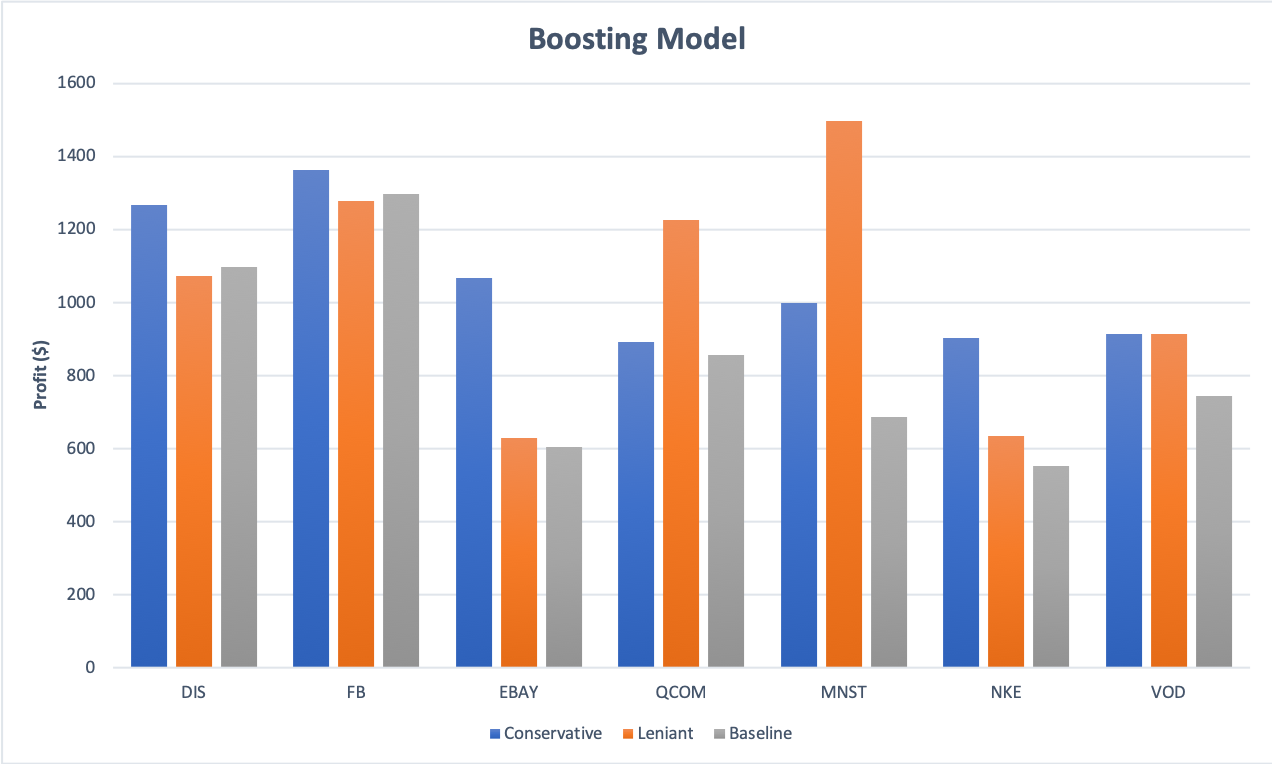
\includegraphics[width=.9\textwidth]{BoostingModelResults.png}
\caption{Stacking Model Results \label{overflow}}
\label{stackingresults}
\end{figure}

\subsection{Deep Learning Model}
Our deep learning model acts differently than any of the above models, as it predicts the price of the following days close. This model has more average performance, but is far more consistent. Rarely does a particular stock trading on the strategy truly perform terribly. Figure~\ref{deepresults} shows our results for some specific stocks within the data. The first 5 stocks in the model, QCOM to MSFT, demonstrate how the strategy hovers close to the baseline and gives consistent performance. Interestingly the last two stocks, EBAY and SBUX, have incredible performance. There is a respective improvement of \$559.53 and \$785.71 for our strategy over the baseline. Given that the initial capital is \$1000, these are some truly astonishing results. 


While we do find far less instances of beating the baseline, our model has far more consistent performance than any of the others discussed above. This is most likely attributed to the accuracy of the predicted stock prices. The RMSE of all of our stocks range between 1.5 and 2.5, signifying that our model is able to predict the closing price of stocks extremely closely. While the predicted price is close, it isn't accurate enough to be consistently profitable. This performance is most likely due the model predicting stock prices for multiple days in a row either above or below the current price, which hampers performance for our end-of-day trading strategy that is entirely reliant on  predictions of price change up or down. Future work could predict multiple days of stock prices in the future and then act on sustained performance rather than specific day-by-day changes to help with this issue in our strategy. 

\begin{figure}[h]
\centering
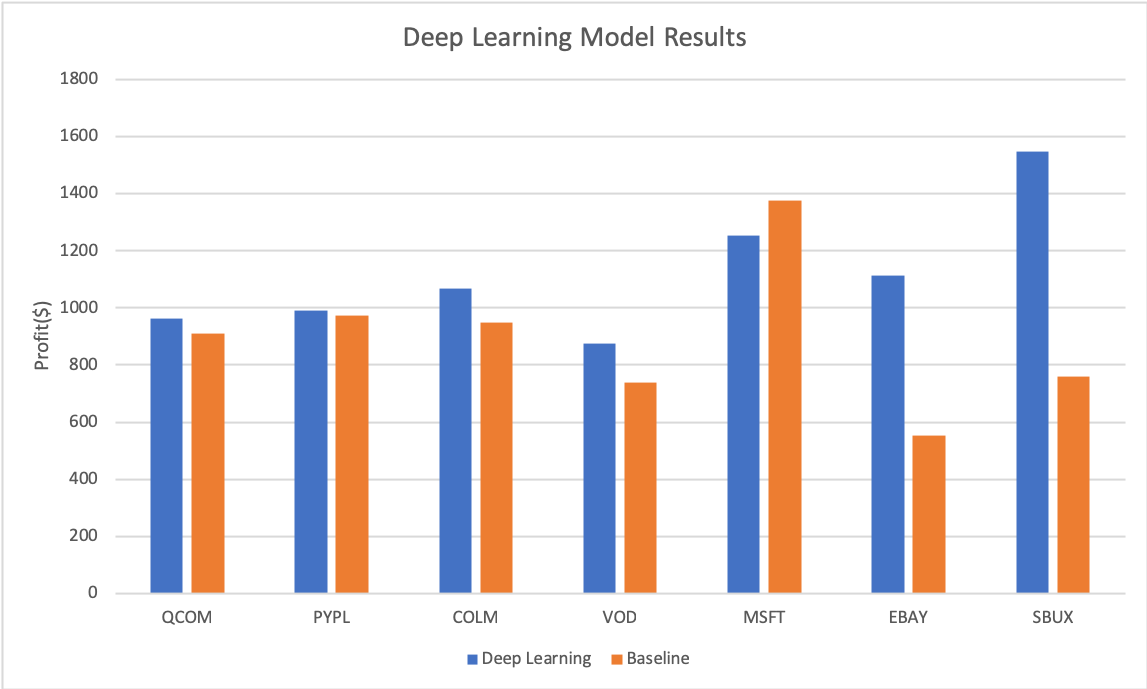
\includegraphics[width=.9\textwidth]{DeepLearningResults.png}
\caption{Deep Learning Model Results \label{overflow}}
\label{deepresults}
\end{figure}


\end{document}
